\documentclass{standalone}
\usepackage{amsfonts, amsmath, amssymb, bm} %Math fonts and symbols
\usepackage{dcolumn, multirow} % decimal-aligned columns, multi-row cells
\usepackage[colorlinks=true]{hyperref}
\usepackage{graphicx, subfigure, float} % graphics commands
\usepackage[margin=1in]{geometry} % sets page layout
\usepackage{setspace}% allows toggling of double/single-spacing
\usepackage{verbatim}% defines environment for un-evaluated code
\usepackage{natbib}% defines citation commands and environments.
\singlespace % set document spacing to single
\bibpunct[, ]{(}{)}{,}{a}{}{,} % sets the punctuation of the bibliography entires.
\newcolumntype{d}[1]{D{.}{.}{#1}} % defines a decimal-aligned column
\usepackage{tikz}
\usetikzlibrary{intersections}
\usepackage{enumerate}
\usepackage[utf8]{inputenc}
\usepackage[english]{babel}
\usetikzlibrary{shapes.geometric}
\hyphenpenalty=10000

\begin{document}
    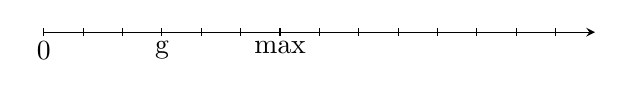
\begin{tikzpicture}[>=stealth]
        \begin{scope}
        \draw [->] (0,0) node [below] {0} -- (1.5,0) node [below] {g} -- (3,0)node [below] {max} -- (6,0) node [below] {} -- (7,0);
        \foreach \x in {0,.5,...,6.5}{
            \draw (\x, -.05) -- (\x, .05);
        }
        \end{scope}
        
    \end{tikzpicture}
\end{document}
